\chapter*{Results}
\label{ch:results}
The performance metrics considered for evaluation in these analysis are the
following: accuracy, precision, recall, and F1-score. Considering all of these
metrics is crucial to accurately evaluate how well each model performs.
Regarding the static models implemented in this project, the classification
report revealed an accuracy of 34\% for the Random Forest algorithm and 24\% for
SVM. These results can be considered reasonable, given that the task at hand
is a multi-class classification problem with 8 classes.\\
For the Random Forest model, the class with the highest F1-score is \texttt{anger},
which is the third class as for support, sitting at 4436. 
\texttt{Joy} was the most supported class, with 5854 instances, but it came second
as for the F1-score, which was of 0.40. The second class based off support, which
was \texttt{fear} with 4652 instances, had a lower F1-score of 0.31. 
The remaining classes showed comparable support and F1-scores, averaging around
3500 instances and 0.25 respectively, only \texttt{disgust} had a considerably
lower F1-score, at 18\%. In image \ref{fig:roc_rf}, the ratio of true positives versus false positives is
displayed, with the Random Forest classifier scoring lower than a random guesser in
two out of eight classes. Image \ref{fig:cwa_rf} shows class-wise accuracy.\\
\begin{figure}[H]
    \centering
    \begin{subfigure}{0.45\textwidth}
        \centering
        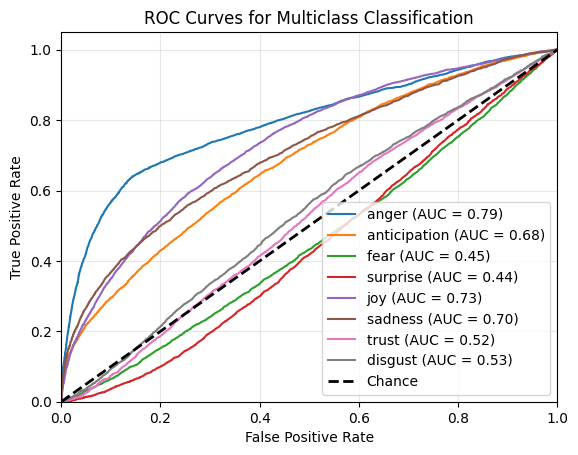
\includegraphics[width=\textwidth]{pictures/roc_rf.png}
        \caption{ROC Curve for the Random Forest Classifier}
        \label{fig:roc_rf}
    \end{subfigure}
    \begin{subfigure}{0.45\textwidth}
        \centering
        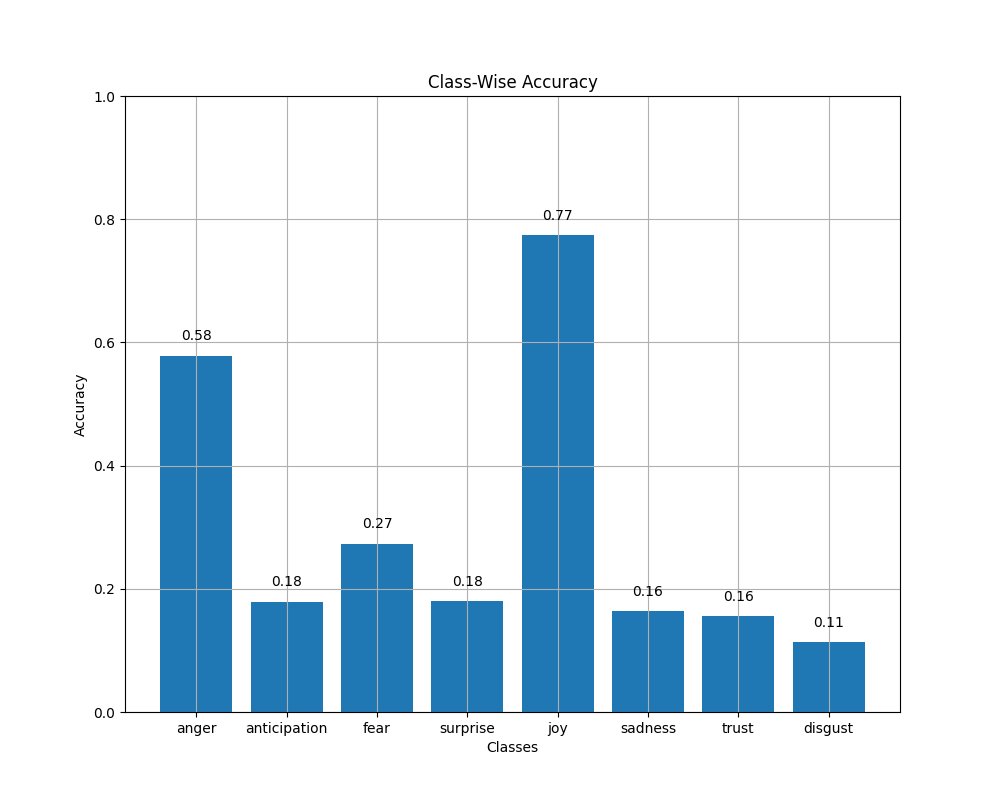
\includegraphics[width=\textwidth]{pictures/class_accuracy.png}
        \caption{Class-wise Accuracy - Random Forest}
        \label{fig:cwa_rf}
    \end{subfigure}
    \caption{Random Forest - plots}
    \label{fig:side_by_side}
\end{figure}

%\begin{figure}[H]
 %   \centering
  %  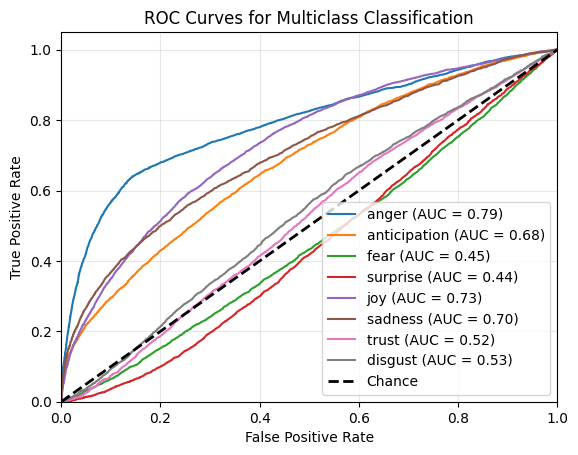
\includegraphics[width=0.5\linewidth]{pictures/roc_rf.png}
   % \caption{ROC Curve for the Random Forest Classifier}
   % \label{fig:roc_rf}
%\end{figure}

%\begin{figure}[H]
 %   \centering
  %  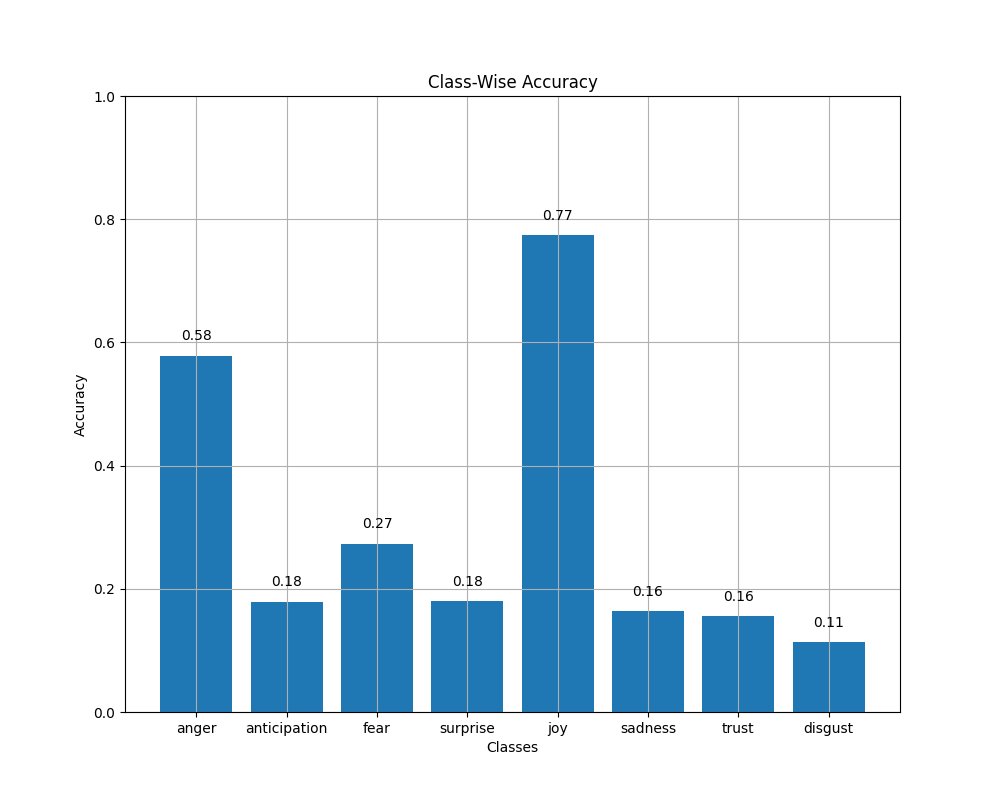
\includegraphics[width=0.5\linewidth]{pictures/class_accuracy.png}
  %  \caption{Class-wise Accuracy - Random Forest}
  %  \label{fig:cwa_rf}
%\end{figure}

For the Support Vector Machine model, the class with the highest F1-score is \textit{fear}, followed by \textit{anger} at 0.31 and \textit{anticipation} at 0.25. 
As for the other classes, the scores were not as comparable as for Random Forest, oscillating between the 22\% of \textit{sadness} and the 7\% of \textit{joy}, with \textit{disgust} and \textit{trust} sitting at 16\%, and \textit{surprise} at 12\%. 
Surprisingly, \textit{joy} is the least performing class for SVC, dispite having the highest support.   
In image \ref{fig:roc_svm}, the ratio of true positives versus false positives is displayed. 
The SVM model performs better than a random guesser in all of the classes, therefore surpassing Random Forest despite the lower scores of accuracy. 
Lastly, image \ref{fig:cwa_svm} shows the class-wise accuracy by SVM, highlighting a clear and strong disparity in the classification performances among the classes.
\begin{figure}[H]
    \centering
    \begin{subfigure}{0.45\textwidth}
        \centering
        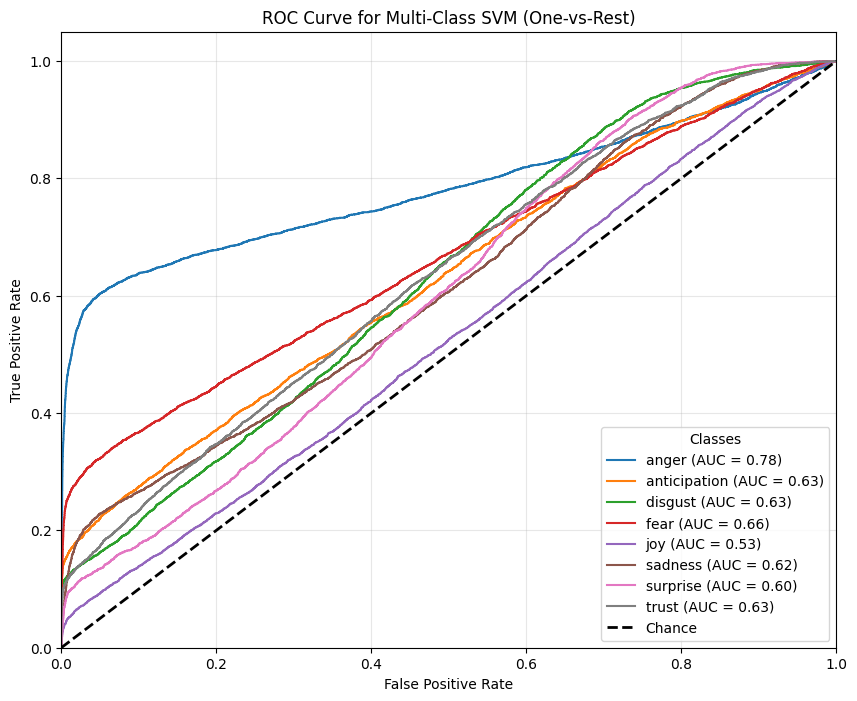
\includegraphics[width=\textwidth]{pictures/roc_svc.png}
        \caption{ROC Curve - SVM}
        \label{fig:roc_svm}
    \end{subfigure}
    \begin{subfigure}{0.45\textwidth}
        \centering
        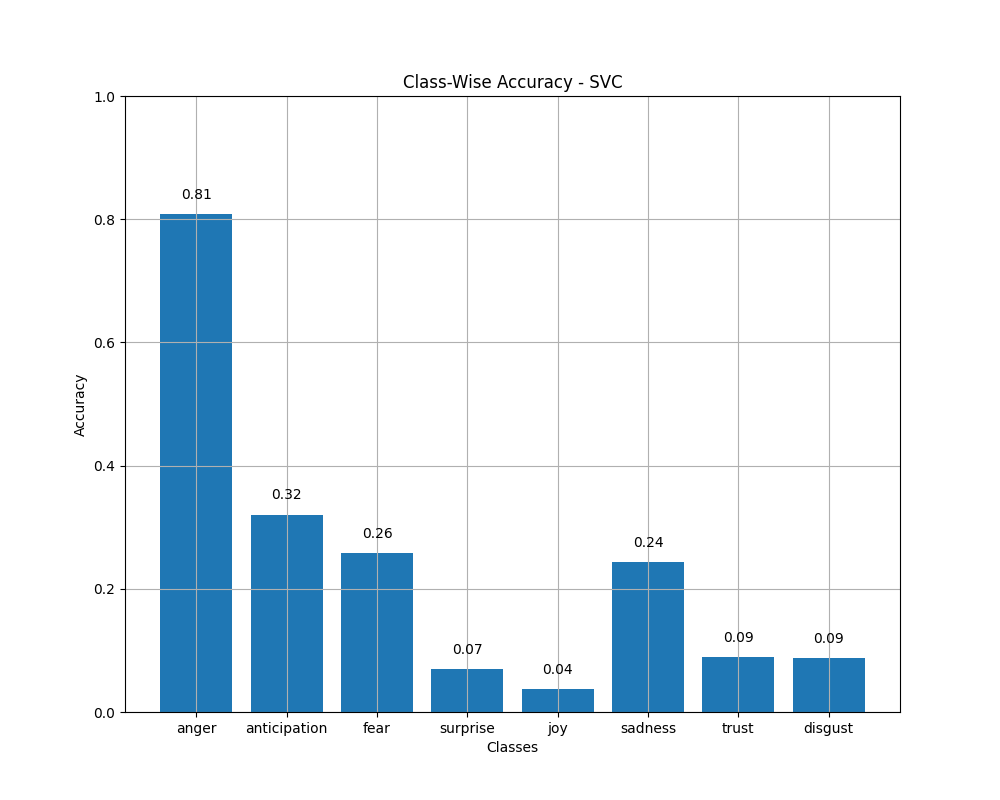
\includegraphics[width=\textwidth]{pictures/class_accuracy_SVC.png}
        \caption{Class-wise Accuracy - SVM}
        \label{fig:cwa_svm}
    \end{subfigure}
    \caption{SVM - plots}
    \label{fig:svm_metrics}
\end{figure}

%\begin{figure}[H]
 %   \centering
%    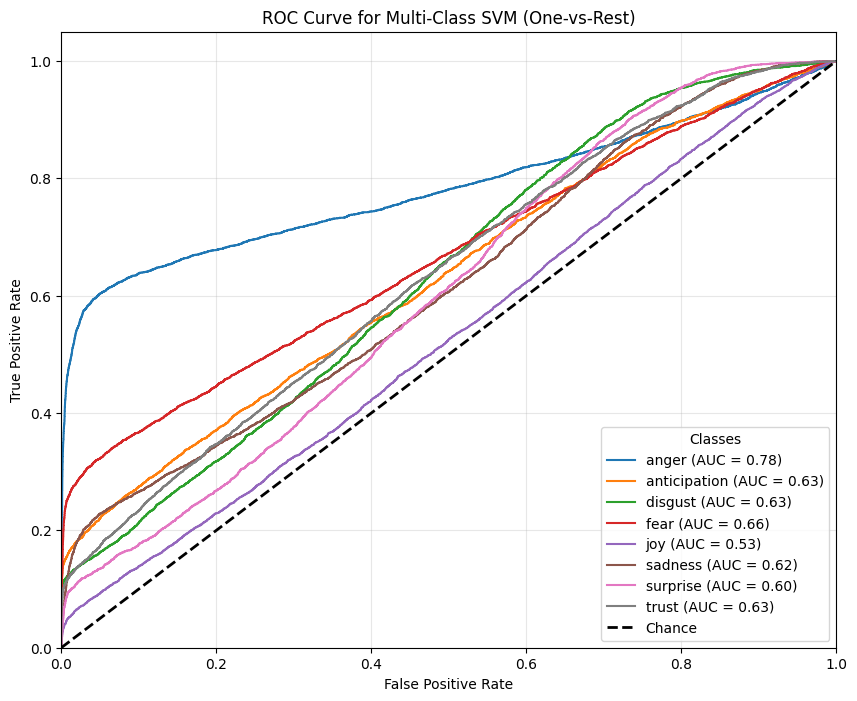
\includegraphics[width=0.5\linewidth]{pictures/roc_svc.png}
 %   \caption{ROC Curve - SVM}
  %  \label{fig:roc_svm}
%\end{figure}
%\begin{figure}[H]
%    \centering
%    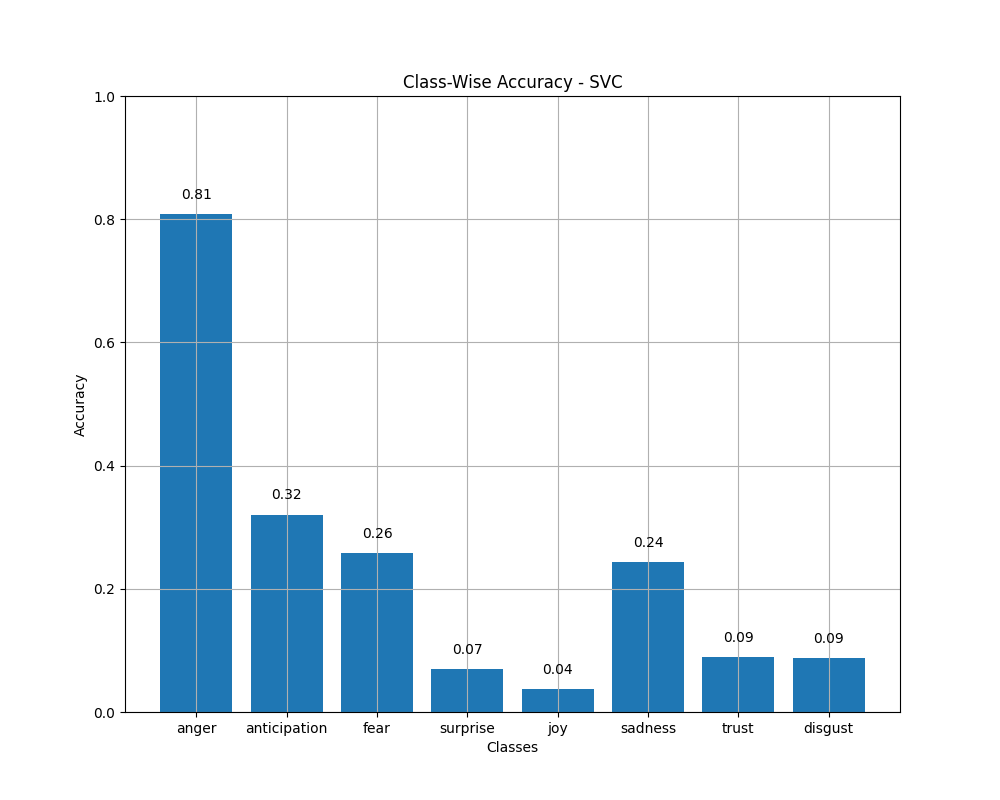
\includegraphics[width=0.5\linewidth]{pictures/class_accuracy_SVC.png}
%    \caption{Class-wise Accuracy - SVM}
%    \label{fig:cwa_svm}
%\end{figure}

As mentioned in the previous chapter, the development of neural networks
iterated testing phases and adjustments over different aspects of training.
Semi-supervised learning through generation of pseudo labels via the partially
trained models generally yielded poor results; on the other hand, downsampling
into evenly represented labels gave some minor improvements, for both architectures.
The neural networks generally underperformed compared to the static models:
the convolutional neural network ultimately reached a test categorical accuracy
of 0.2128, while the recurrent neural network had a test accuracy of \textbf{MANCA QUALCOSA}. \\
The graphs below show various performance metrics of the network with the better
performances for the convolutional architecture.
\begin{figure}[H]
    \centering
    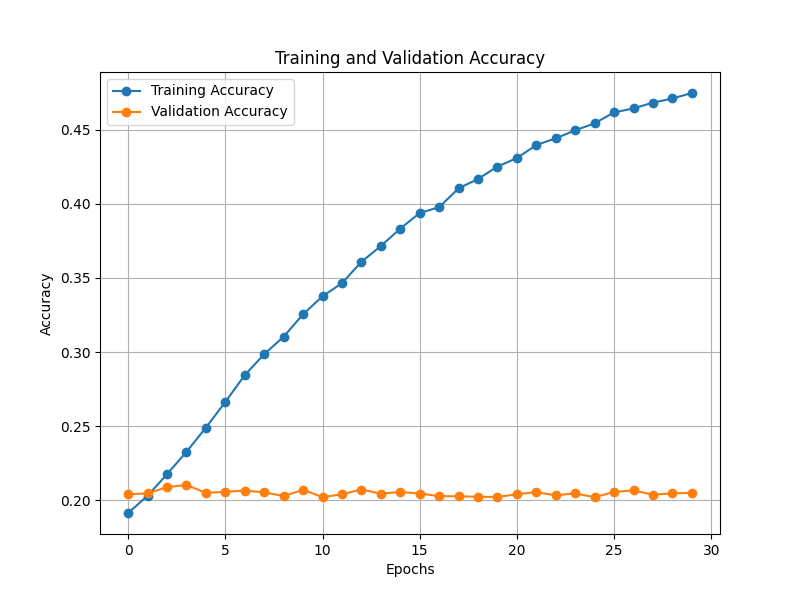
\includegraphics[width=0.40\linewidth]{pictures/cnn_accuracy.png}
    \caption{Convolutional Neural Network's training and validation accuracy}
    \label{fig:cnn_train_val_acc}
\end{figure}

\begin{figure}[H]
    \centering
    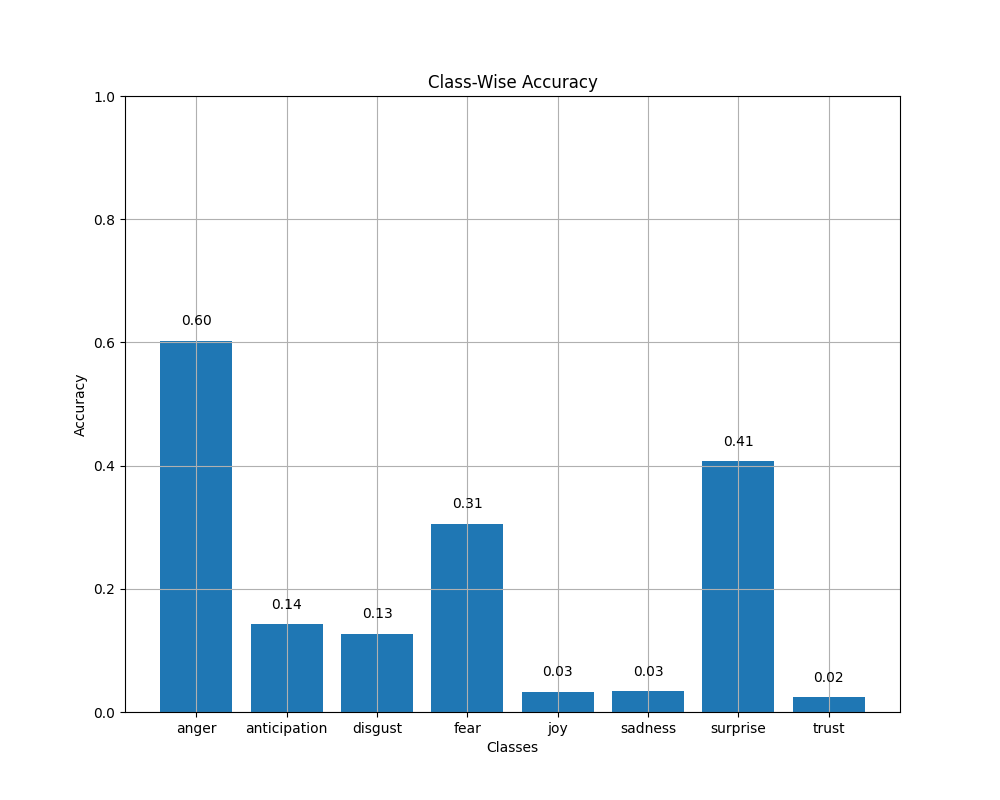
\includegraphics[width=0.65\linewidth]{pictures/cnn_class_accuracy.png}
    \caption{Convolutional Neural Network's class-wide accuracy}
    \label{fig:cnn_classacc}
\end{figure}

\begin{figure}[H]
    \centering
    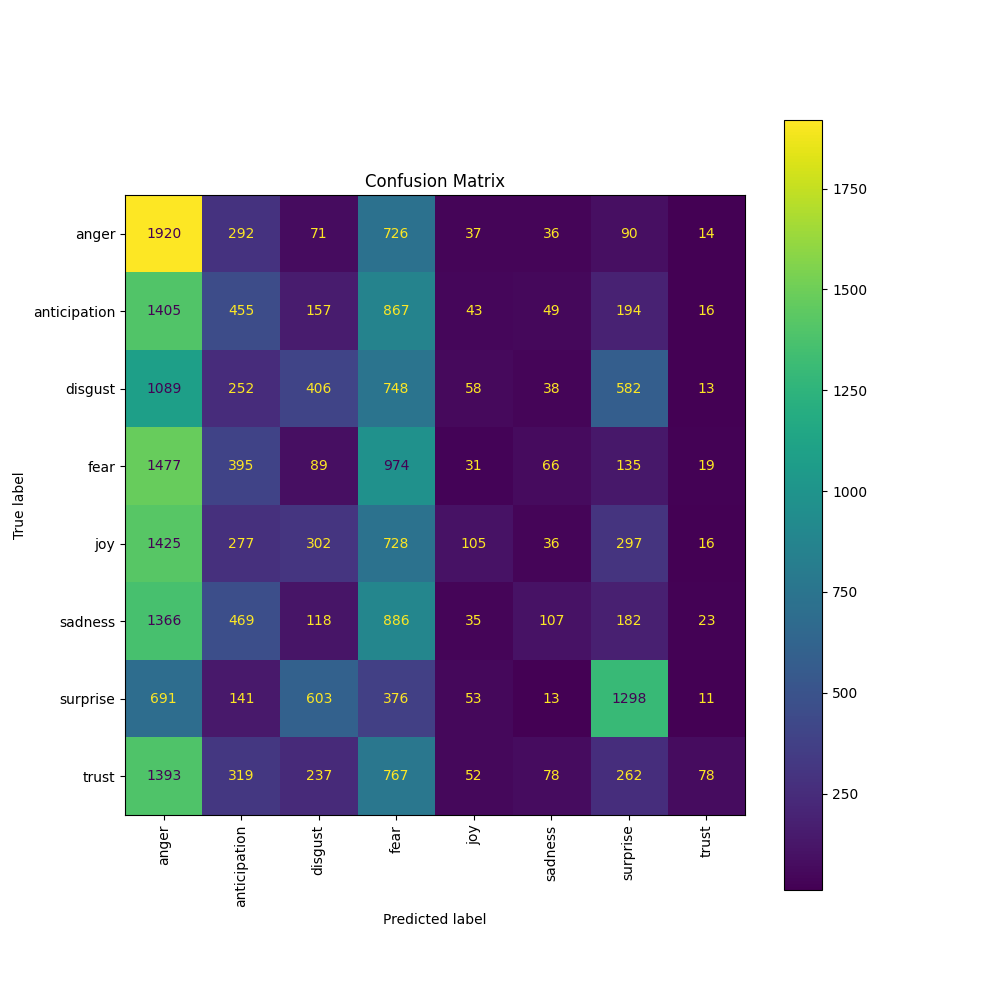
\includegraphics[width=0.65\linewidth]{pictures/cnn_confusion_matrix.png}
    \caption{Convolutional Neural Network's confusion matrix}
    \label{fig:cnn_confmatr}
\end{figure}

The graphs below show various performance metrics of the network with the better
performances for the recurrent architecture \textbf{GRAFICI RECURRENT}.
% TODO

% Judging from the confusion matrices
% and training and validation accuracy plots, the models tend to confuse the classes.
% This might be because of heavy high frequency overlapping terms between the classes